\documentclass[12pt, a4paper]{book}
\begin{document}
The Standard Model (SM) of particle physics is the framework of particle physics, it unveils the secrets of the universe's building blocks and their interactions. With its framework, it offers a rich understanding 
of the structure and behavior of matter, solidifying its place as a bedrock in the realm of modern physics. At its core, the Standard Model describes three of the fundamental forces of nature: the electromagnetic force, 
the weak force, and the strong force. These forces are mediated by particles known as gauge bosons, which act as carriers of the forces between matter particles.\\
\\As the SM is described using Quantum Field Theory (QFT), we need the description of what a \textit{field} is. A quantum field is a fundamental concept in quantum physics that describes the underlying fabric of reality, 
where particles and their interactions are represented as excitations or vibrations of these fields. In this chapter we will delve into every of the aforementioned forces, the spontaneous symmetry breaking phenomenum that 
gives mass to particles, as well as how to calculate the cross-section of processes. We will start by describing electromagnetism in terms of QFT, namely Quantum Electrodynamics.\\
\\The theory of this section is mainly based on Peskin's and Schroeder's "An Introduction to Quantum Field Theory" \cite{Peskin:1995ev} and partly on Thomson's "Modern Particle Physics" \cite{THOMSON}.

\clearpage
\section{Quantum Electrodynamics}
In the beginning there was nothing; \textit{then God said, “Let there be light,” and there was light.} The first part of the Standard Model, Quantum Electrodynamics, or QED for short, described the processes in nature involving the photon. 
The Lagrangian of QED can be seen below
\begin{equation}\label{eq:QED}
    \mathcal{L}_{QED} = \overline{\psi}\left(i\slashed{D} -m\right)\psi -\frac{1}{4}B^{\mu\nu}B_{\mu\nu}
\end{equation}
with $\overline{\psi}=\psi^\dagger\gamma^0$, where $\psi$ is a bispinor field of spin-1/2\footnote{In QED, it is the electron or positron field}, $m$ is the mass of $\psi$, $\gamma^\mu$ are the Dirac matrices, defined as 
$$
\begin{aligned}
    \gamma ^{0}&={\begin{pmatrix}1&0&0&0\\0&1&0&0\\0&0&-1&0\\0&0&0&-1\end{pmatrix}},&\gamma ^{1}&={\begin{pmatrix}0&0&0&1\\0&0&1&0\\0&-1&0&0\\-1&0&0&0\end{pmatrix}},\\\\
    \gamma ^{2}&={\begin{pmatrix}0&0&0&-i\\0&0&i&0\\0&i&0&0\\-i&0&0&0\end{pmatrix}},&\gamma ^{3}&={\begin{pmatrix}0&0&1&0\\0&0&0&-1\\-1&0&0&0\\0&1&0&0\end{pmatrix}}~
\end{aligned}
$$
Furthermore we have $\slashed{D}\equiv \gamma^\mu D_\mu$ where $iD_\mu = i\partial_\mu -eB_\mu$ is the covariant derivative, where $e$ is the coupling constant\footnote{Which in QED is the electric charge of $\psi$.},
$B_{\mu\nu}=\partial_\mu B_\nu - \partial_\nu B_\mu$ is the electromagnetic field tensor\footnote{Taking $\partial_\mu B^{\mu\nu} + \star \partial_\mu B^{\mu\nu} = 0$ gives all of Maxwell's equations.}. 
$B_\mu$ is the covariant four-potential\footnote{Defined as $B_\mu = (\frac{1}{c}\phi, \mathbf{B})$ where $\phi$ is the electric potential and $\mathbf{B}$ is the magnetic potential we know and love from electrodynamics. } of the electromagnetic field, also known as the gauge field.\\ 
\\The above Lagrangian is described by a $U(1)$ symmetry group, meaning that it corresponds to the $unitary$ group of one unitary matrix with determinant 1\footnote{For more information about group theory we refer the reader to Georgi's "LIE ALGEBRAS IN PARTICLE PHYSICS. FROM ISOSPIN TO UNIFIED THEORIES" \cite{Georgi:1982jb}}. 
The consequence of QED being described by this symmetry group is, recalling Noether's theorem, that there is only one unique degree of freedom, this is the rotation of phase angle, $\alpha(x)$, of the field $\psi$. This means that 
\begin{equation}\label{eq:gauge_psi}
    \psi \rightarrow \psi' = e^{ie\alpha}\psi
\end{equation}
% and 
% \begin{equation}
%     B_\mu \rightarrow B_\mu' = \frac{1}{e}D_\mu\alpha
% \end{equation}
Inserting $\psi'$ into the Eq. (\ref{eq:QED}) yields that $\mathcal{L}\rightarrow\mathcal{L}'=\mathcal{L}$, meaning that our theory is locally gauge invariant.

\section{Yang-Mills Theory}
While QED is expressed by the Lagrangian in Eq. (\ref{eq:QED}), which is part of a $U(1)$ symmetry group, it can still be described by a more general Lagrangian using \textit{Yang-Mills} theory.
The differences between the Yang-Mills and QED Lagrangian being that the gauge freedom changes from a plane rotation of the phase angle $\alpha$ of the field $\psi$, to a more general
gauge in $\alpha^a$ in the field $f_i$ (using now the infinitesimal transformation notation)
$$
    f_i \rightarrow \left(1+ig \alpha^a t^a + \mathcal{O}(\alpha^2)\right) f_i    
$$
The covariant derivative also changes to a more general 
$$
iD_\mu = i\partial_\mu -eB_\mu\rightarrow iD_\mu = i\partial_\mu -gA^a_\mu t^a
$$
where $e$ is replaced by a coupling constant $g$, the vector field $B_\mu$ changes to a more general $A_\mu^a$ which transforms as 
$$
A_\mu^a \rightarrow A^a_\mu +\frac{1}{g}\partial_\mu\alpha^a +f^{abc}A_\mu^b\alpha^c
$$
where $f^{abc}$ is a set of numbers called the \textit{structure constants}. 
The important thing to note about the Yang-Mills is that the covariant derivative is \textit{non-Abelian}\footnote{Except in the trivial case where we use the $U(1)$ symmetry group}, meaning that the commutator of the operator becomes
$$
\left[D_\mu,D_\nu\right] = -igF_{\mu\nu}^at^a
$$
this new $t^a$ factor is a Lie algebra generator, which for our purposes represent a local gauge symmetry we have on the field. The structure constant has to fulfill the criteria that
\begin{equation}\label{eq:struc_const}
    [t^a,t^b]=if^{abc}t^c
\end{equation}
The difference between the Yang-Mills and the QED Lagrangian is most noticeable when fully writing
$$
F_{\mu\nu}^a = \partial_\mu A_\nu^a -\partial_\nu A_\mu^a +gf^{abc}A_\mu^b A_\nu^c
$$
Where the last term takes into account the \textit{self interaction} of bosons. Adding all of this up we get the following Lagrangian
\begin{equation}\label{eq:YM_lag}
    \mathcal{L}_{YM} = \overline{f}\left(i\slashed{D} -m\right)f -\frac{1}{4}F^a_{\mu\nu}F^{\mu\nu}_a
\end{equation}
where we use the notation $f\equiv\begin{pmatrix}f_1&f_2&\cdots&f_n\end{pmatrix}^T$ where $f_i$ is a field. 
Using the Euler-Lagrange equation with the Yang-Mills Lagrangian above yields the equation of motion
\begin{equation}\label{eq:YM_eq}
    \partial^\mu F^a_{\mu\nu} +gf^{abc}A^{b\mu}F^c_{\mu\nu} = -g\overline{\psi}\gamma_\nu t^a\psi
\end{equation}
As using Noether's theorem on the equation of motion gives us the conserved quantity of the theory, we will apply it for every symmetry group in the SM. There is also a theorem\footnote{See Georgi's book \cite{Georgi:1982jb}} that states that for an $SU(n)$ symmetry group there are $n^2-1$ vector fields.\\
\\If we were to choose $U(1)$ as our local symmetry group the generator $t^a = \mathbb{I}$ and all the structure constants are $f^{abc}=0$, meaning that we get the QED back. 
Noether's theorem states that the conserved quantity of the Lagrangian is the electric charge $e$.

\clearpage
\section{Weak theory}
Using the Yang-Mills Lagrangian from Eq. (\ref{eq:YM_lag}) on $SU(2)$, choosing $t^a =\frac{\sigma^i}{2}$, where $\sigma^i$ are the Pauli matrices given as 
\begin{align}\label{eq:Pauli}
    \begin{split}
        \sigma ^{1}={\begin{pmatrix}0&1\\1&0\end{pmatrix}},\quad 
        \sigma ^{2}={\begin{pmatrix}0&-i\\i&0\end{pmatrix}},\quad 
        \sigma ^{3}={\begin{pmatrix}1&0\\0&-1\end{pmatrix}}
    \end{split}
\end{align} 
The structure constants are the Levi-Civita $f^{abc}=\epsilon^{ijk}$. Where $i,j,k\in[1,2,3]$.
The Weak theory gives us the gauge freedoms of
$$
f \rightarrow \left(1+i \alpha^i \sigma^i + \mathcal{O}(\alpha^2)\right) f
$$ 
Using the notation of $A_\mu\rightarrow W_\mu$ we get that there are $2^2-1$, meaning three vector fields 
$$
W_\mu^i \rightarrow W^i_\mu +\frac{1}{g}\partial_\mu\alpha^i +\epsilon^{ijk}W_\mu^j\alpha^k
$$
We cannot directly apply Noether's theorem on this Lagrangian, as it is not renormalizable, but when arriving to \textit{electroweak} theory we would get that two quantities are conserved\footnote{See Section \ref{sec:EW}}, the \textit{hypercharge} and \textit{isospin}. 
In this theory we have isospin doublets, meaning 
$$
f=\begin{pmatrix}
    f_1\\f_2
\end{pmatrix}
\rightarrow \begin{pmatrix}
    U\\D
\end{pmatrix}
$$
For \textit{up and down type} particles. i.e. $\begin{pmatrix}
    l\\\nu_l
\end{pmatrix}$ for leptons, and $\begin{pmatrix}
    u\\d
\end{pmatrix}$ for quarks.


\section{Quantum Chromodynamics}
Using the Yang-Mills Lagrangian from Eq. (\ref{eq:YM_lag}) on an $SU(3)_C$, choosing $t^a =\frac{\lambda^a}{2}$, where $\lambda^a$, the \textit{Gell-Mann matrices}, are the $SU(3)$ equivalent of the $SU(2)$ Pauli matrices:
\begin{align}\label{eq:Gell-Mann}
    \begin{split}
        \lambda ^{1}={\begin{pmatrix}0&1&0\\1&0&0\\0&0&0\end{pmatrix}},\quad 
        \lambda ^{2}={\begin{pmatrix}0&-i&0\\i&0&0\\0&0&0\end{pmatrix}},\quad 
        \lambda ^{3}={\begin{pmatrix}1&0&0\\0&-1&0\\0&0&0\end{pmatrix}}, \\\\
        \lambda ^{4}={\begin{pmatrix}0&0&1\\0&0&0\\1&0&0\end{pmatrix}},\quad 
        \lambda ^{5}={\begin{pmatrix}0&0&-i\\0&0&0\\i&0&0\end{pmatrix}},\quad 
        \lambda ^{6}={\begin{pmatrix}0&0&0\\0&0&1\\0&1&0\end{pmatrix}}, \\\\
        \lambda ^{7}={\begin{pmatrix}0&0&0\\0&0&-i\\0&i&0\end{pmatrix}},\quad 
        \lambda ^{8}={\frac {1}{\sqrt {3}}}{\begin{pmatrix}1&0&0\\0&1&0\\0&0&-2\end{pmatrix}}
    \end{split}
\end{align} 
The structure constant have to obey Eq. (\ref{eq:struc_const}), thus we get 
\begin{align*}
    f^{123}=1\\
    f^{147}=-f^{156}=f^{246}=f^{257}=f^{345}=-f^{367}={\frac{1}{2}}\\
    f^{458}=f^{678}={\frac {\sqrt {3}}{2}}
\end{align*}
Using the notation of $A_\mu\rightarrow G_\mu$ we get that there are $3^2-1$, meaning \textit{eight} vector fields 
$$
G_\mu^a \rightarrow G^a_\mu +\frac{1}{g_s}\partial_\mu\alpha^a +\epsilon^{abc}G_\mu^b\alpha^c
$$
If one were to use Noether's theorem on the $SU(3)_C$ Yang-Mills Lagrangian, we would get that there are three conserved quantities for this symmetry group. These are the colors, $r,g$ and $b$. With all the information above we can 
fully describe Quantum Chromodynamics, which describe quark interactions. The eight vector fields are the eight different gluons that are in the theory.\\
\\In this theory we have color triplets
$$
f=\begin{pmatrix}
    f_1\\f_2\\f_3
\end{pmatrix}
$$
where $f_i$ is the color state of the particle we are studying.

\section{Electroweak unification and the BEH Mechanism}\label{sec:EW}
We have so far introduced the three symmetry groups that form the SM, but this is not the full picture yet. To get the full SM we need to talk about the electroweak $U(1)_Y\otimes SU(2)_L$ unification as proposed by Glashow-Weinberg-Salam, 
which in turn yields four massless vector fields (three $W_i$ from $SU(2)_L$, and $B$ from $U(1)$). The universe we observe however, does not have four such vector fields, the $W^\pm$ and $Z$ are massive, and in fact only the photon is 
massless.\\
\\As proposed by Higgs-Braut-Englert we can introduce a complex scalar $\phi$, which is charged under $SU(2)_L\otimes U(1)_Y$ with a hypercharge of $1/2$. This leads to the general, renormalizable Lagrangian 
\begin{equation}\label{eq:electroweak}
    \mathcal{L}\supset \mathcal{L}_\phi = \left(D_\mu \phi\right)^\dagger\left(D^\mu \phi\right) -\mu^2\left(\phi^*\phi\right) - \lambda^2\left(\phi^*\phi\right)%-\lambda\left(\phi^\dagger \phi -\frac{v^2}{2}\right)^2
\end{equation}
with 
\begin{equation}\label{eq:covar_higgs}
    D_\mu \phi =\partial_\mu \phi -igW_\mu^a\sigma^a-ig'y_\phi \phi
\end{equation}
where $W_\mu$ and $B_\mu$ are vector fields of the $SU(2)_L$ and $U(1)_Y$ group respectively. And where $\mu^2\left(\phi^*\phi\right) - \lambda^2\left(\phi^*\phi\right)= V(\phi)$ is the potential of the new complex scalar field. Expanding about this
potential with a real scalar field then yields the Higgs doublet, written in unitary gauge 
\begin{equation}\label{eq:Higgs}
    \phi = \begin{pmatrix}
        0\\v+H(x)
    \end{pmatrix}
\end{equation}
where $H$ is real scalar field. This expands the potential to be
\begin{equation}\label{eq:sombrero}
    V(H) =\frac{1}{2}m_H^2H^2 + \frac{1}{2v}m_H^2H^3 +\frac{1}{8v^2}m_H^2H^4
\end{equation}
where we have used that $m_H = \sqrt{2\lambda}v$. This potential is the so-called \textit{Sombrero potential}, and we can reveal that this scalar field $H$ is the Higgs boson. 
In choosing unitary gauge, meaning Eq. (\ref{eq:Higgs}), we have seemingly removed three degrees of freedom from the Lagrangian. To see where the degrees of freedom have gone, we return to the Lagrangian in Eq. (\ref{eq:electroweak}) and write out
Eq (\ref{eq:covar_higgs}), which (after a lot of math) yields the following new fields
\begin{equation}\label{eq:W_boson}
    W_\mu^\pm = \frac{W_\mu^1 \mp iW_\mu^2}{\sqrt{2}}
\end{equation}
\begin{equation}\label{eq:Z_boson}
    Z_\mu = \frac{gW_\mu^3 - g'B_\mu}{\sqrt{g^2+e^2}}
\end{equation}
\begin{equation}\label{eq:photon}
    A_\mu = \frac{gB_\mu - g'W_\mu^3}{\sqrt{g^2+e^2}}
\end{equation}
These are the $W$ and $Z$ boson as well as the photon, respectively. The three degrees of freedom we lost on the unitary gauge went to give mass to the $W^+$, $W^-$ and $Z$, while the photon remains massless.\\
\\To explicitly show how the SSB phenomena gives mass to every other particle, one can transform the Lagrangian to the unitary gauge, 
this adds an extra term on the Lagrangian called the $Yukawa$ Lagrangian
$$
\mathcal{L}_{YU} = \psi_i y_{ij}\psi_j\phi
$$
where $y_{i,j}$ are the Yukawa couplings between the scalar, $\phi$, and fermion field, $\psi$. As we are looking at a complex scalar field in the $SU(2)$ representation we have from the Yang-Mills theory
$$
f=\begin{pmatrix}
    U\\D
\end{pmatrix}
$$
where $U,D$ is the field \textit{up and down type} spinor. For example this can be the first generation quark two component spinor $Q = \begin{pmatrix}
    u\\ d
\end{pmatrix}$ consisting of the $up$ and $down$ quark or the lepton two component spinor $L = \begin{pmatrix}
    l\\ \nu_l
\end{pmatrix}$. The standard for weak interactions is to define $right$ and $left$ handed helicity using the operators 
$$
L = \frac{1}{2}(\mathbb{I} - \gamma_5),\qquad\text{and}\quad R = \frac{1}{2}(\mathbb{I} + \gamma_5)
$$
where $\gamma_{5}=i\gamma^0\gamma^1\gamma^2\gamma^3$. Such that we can write 
$$
U_L = L\begin{pmatrix}
    U\\D
\end{pmatrix} = \begin{pmatrix}
    U\\0
\end{pmatrix},\qquad\text{and}\quad D_R = R\begin{pmatrix}
    U\\D
\end{pmatrix} = \begin{pmatrix}
    0\\D
\end{pmatrix}
$$
as well as their hermitian conjugates. 


\section{S-matrix expansion}
But how do we predict the occurrences of processes? To explain this generally, we can conduct an S-matrix expansion. To be more precise and use terms from quantum field theory rather than quantum mechanics, we can use the scattering operator $\mathcal{S}$ on the interaction 
term of the SM Lagrangian $\mathcal{L}_{int}$. Starting by defining the general operator
\begin{align}\label{eq:S-matrix}
    \begin{split}
        \mathcal{S} = \sum_{i = vertices}\mathcal{S}^{(i)},\qquad\text{where}\quad \mathcal{S}^{(0)} = \mathbb{I}\qquad\text{and}\quad \\
        \mathcal{S}^{(n)}=(-i)^n\mathcal{T}\int_{-\infty}^{\infty}d^4\mathbf{x}_1\cdots\int_{-\infty}^{\infty}d^4\mathbf{x}_n\left[\mathcal{L}_{int}(x_1)\cdots\mathcal{L}_{int}(x_n)\right]
    \end{split}
\end{align}
where $\mathcal{T}$ is the \textit{time operator} ordering the terms such that we predict our desired transition amplitude, and $\mathbf{x}_i$ are coordinates in spacetime.  The $\mathcal{S}$ operator sums over all \textit{vertices} 
of a \textit{Feynman diagram}. To calculate the probability amplitude we can start with an easy example using QED, the Bhabha scattering process $e^- e^+\rightarrow e^-e^+$, in particular the annihilation channel where we have $e^+e^-\rightarrow\gamma$ on a vertex level. The interaction Lagrangian of interest for this process is
$\mathcal{L}_{int} = e\overline{\psi}(x)\gamma^\mu\psi(x)A_\mu$. We use the scattering operator in the following way
$$
\bra{f}\mathcal{S}^{(n)}\ket{i} \rightarrow \bra{e^-e^+}S^{(2)}\ket{e^-e^+} 
$$
$$
= \bra{e^-e^+}\left(-e^2\mathcal{T}\int_{-\infty}^{\infty}d^4\mathbf{x} \int_{-\infty}^{\infty}d^4\mathbf{y} \overline{\psi}(x)\gamma^\mu\psi(x)A_\mu(x)\overline{\psi}(y)\gamma^\nu\psi(y)A_\nu(y) \right)\ket{e^-e^+}
$$
Starting by using the time operator $\mathcal{T}$ on the integrals, which gives us the \textit{normal order} of the operations, we can start by using \textit{Wicks theorem} to "connect" the two points in spacetime $\mathbf{x}$ and $\mathbf{y}$. As we know there are no photons in the initial or final state, we can connect the photons as \textit{propagators}, meaning
$$
\mathcal{S}^{(2)} = -\frac{e^2}{2}\int_{-\infty}^{\infty}d^4\mathbf{x} \int_{-\infty}^{\infty}d^4\mathbf{y} \mathcal{N} \left(\wick{\overline{\psi}(x)\gamma^\mu\c1A_\mu(x)\psi(x)\overline{\psi}(y)\gamma^\nu\c1A_\nu(y)\psi(y)}\right)
$$
where 
$$
\wick{\c1A_\mu(x)\c1A_\nu(y)} = \bra{0}\mathcal{T}(A_\mu(x)A_\nu(y))\ket{0} = \cdots = D_{\mu\nu}^F(x-y) = \int_{-\infty}^{\infty}\frac{d^4q}{(2\pi)^4}D_{\mu\nu}^F(q)e^{-iq(x-y)}
$$
with
\begin{equation}\label{eq:p-prop}
    D_{\mu\nu}^F(k) = \frac{-g_{\mu\nu}+r_{\mu\nu}}{(q^2+i\epsilon)},
\end{equation}
where $q = q_\mu q^\mu$ is the contracted four-momentum of the particle, and $r_{\mu\nu}=\frac{q_\mu q_\nu}{q^2}$ we will set to zero as we will use the Feynman gauge. Here we have omitted the mathematical details, but to summarize it with words. We calculated the photon propagator which connects two spacetime points $\mathbf{x}$ and $\mathbf{y}$ by calculating the Greens function of the Minkowski space using among other the residue theorem from complex analysis. 
If we were now to define $\ket{e^-e^+}, \bra{e^-e^+}, \overline{\psi}$ and $\psi$ we could directly calculate the scattering amplitude by setting in the values, as this usually involves solving integrals that use Dirac delta function\footnote{At least while omitting loops, which we will do in this thesis}. 
To complete our example we define
$$
\ket{e^-e^+} = (\sqrt{2E_p}a^\dagger_{p})(\sqrt{2E_k}b_{k})\ket{0},\qquad\text{and}\quad \bra{e^-e^+} = (2\sqrt{E_pE_k})\bra{0}a_{p}b^\dagger_{k}
$$
where $E_i$ is the energy of the particle and $a_i,b_i$ and $a^\dagger_i,b^\dagger_i$ are creation and annihilation operators, respectively. In general fermion fields have
$$
\psi \equiv\int\frac{d^3p}{(2\pi)^3}\frac{1}{\sqrt{2E_\mathbf{p}}}\left(\sum_sa^s_\mathbf{p}u^s(p)e^{-ip\cdot x}+b^{s\dagger}_\mathbf{p}v^s(p)e^{ip\cdot x}\right) =\psi^+_p+\psi^-_p
$$
Where, depending on $\psi^+$ (for $u(p)$) and $\psi^-$ (for $v(p)$) are the particle and antiparticle fields, respectively. It is standard convention to say that ingoing particles and anti-particles 
on an interaction are written as $\psi^+$ and $\overline{\psi}^-$, respectively, and their hermitian conjugate when they are outgoing. With this information we can connect the initial and final particles to their fields, solving the bra we have
$$
\bra{e^-e^+}\overline{\psi}(x)\psi(x) = (2\sqrt{E_pE_k})\bra{0}a_{p}b^\dagger_{k}\overline{\psi}^-_{k'}\psi^+_{p'},
$$
Giving
$$
\textstyle\bra{e^-e^+}\overline{\psi}(x)\psi(x) = \bra{0} \int\frac{d^3p'}{(2\pi^3)}\int\frac{d^3k'}{(2\pi^3)}\sqrt{\frac{E_pE_k}{E_{p'}E_{k'}}} \left(\sum_{s,t}a^{\dagger,s}_\mathbf{p'}u^s(p')e^{-ip'\cdot x} + b^{t}_\mathbf{k'}\overline{v}^t(k')e^{-ik'\cdot x}\right)a_{p}b^\dagger_{k}
$$
using the relation $a_{p's}a_{pt}^\dagger = (2\pi)^2\delta^{(3)}(p'-p)- a_{p's}^\dagger a_{pt}$ where the latter part kills vacuum, we get
$$
\bra{e^-e^+}\overline{\psi}(x)\psi(x) = u(x)\overline{v}(x)\bra{0}
$$
Doing the same for the ket, and setting all of this into the initial equation we get
$$
\bra{f}\mathcal{S}^{(n)}\ket{i} = -\frac{e^2}{2}\bra{0}\int_{-\infty}^{\infty}d^4\mathbf{x} \int_{-\infty}^{\infty}d^4\mathbf{y} u(x)\gamma^\mu\overline{v}(x)D_{\mu\nu}^F(x-y)\overline{u}(y)\gamma^\nu v(y)\ket{0}
$$
Giving us
$$
(2\pi)^4\delta^{(4)}(p_1+p_2-p'_1-p'_2)\overline{v}(p_1)\gamma^\mu u(p_2) \frac{g_{\mu\nu}}{q^2}\overline{u}(p'_1)\gamma^\nu v(p'_2)
$$
we can relate the scattering amplitude to a variable called the \textit{transition amplitude}, $\mathcal{M}_{fi}$ by using 
$$
\bra{f}\mathcal{S}\ket{i} = i(2\pi)^4\delta^{(4)}\left(\sum_i p_i -\sum_f p_f\right)\mathcal{M}_{fi}
$$
Meaning that we have
$$
\mathcal{M}_{bhabha} = \overline{v}(p_1)\gamma^\mu u(p_2) \frac{g_{\mu\nu}}{q^2}\overline{u}(p'_1)\gamma^\nu v(p'_2)
$$
The reason we did all this is to calculate the \textit{differential cross-section} (in the center of mass frame) from this, using
\begin{equation}\label{eq:diff_cross}
    \frac{d\sigma}{d\Omega} = \frac{1}{64\pi^2s}\frac{p_f*}{p_i*}\abs{\mathcal{M}_{fi}}^2
\end{equation}
where $p_f*$ and $p_i*$ are the magnitudes of the final- and initial-state momenta, respectively. From the differential cross-section we can also calculate the cross-section by integrating over $d\Omega$. 
\begin{equation}\label{eq:cross_sec}
    \sigma = \int_{0}^{2\pi}\int_{0}^{\pi}\frac{1}{64\pi^2s}\frac{p_f*}{p_i*}\abs{\mathcal{M}_{fi}}^2 \sin\theta d\theta d\phi
\end{equation}
This method is a general way to calculate the cross-section of an event we want to study, but usually one just constructs the matrix element $\mathcal{M}_{fi}$ from \textit{Feynman diagrams}. In this calculation we 
already introduced the photon propagator in Eq. (\ref{eq:p-prop}), and we implicitly simplified it to be $\frac{g_{\mu\nu}}{q^2}$, which is valid for our purposes, and can be used in any event where the photon is the propagator. 
Feynman realized this and made Feynman rules to construct diagrams. The rules are shown in Figure \ref{fig:feynman_rules}. \\
\\Meaning that following these rules we just constructed the Feynman diagram for Bhabha scattering shown in Figure \ref{fig:bhabha}
\begin{figure}[!ht]
    \centering
    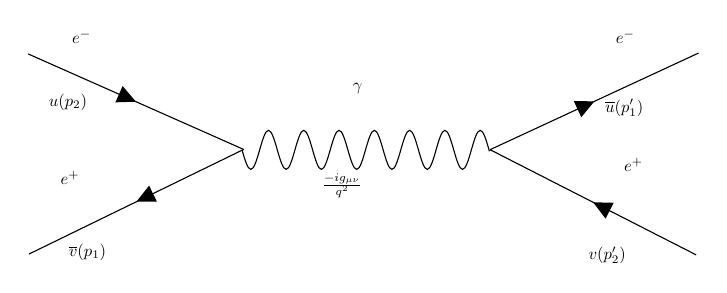
\begin{tikzpicture}[x=0.75pt,y=0.75pt,yscale=-1,xscale=1]
        %uncomment if require: \path (0,261); %set diagram left start at 0, and has height of 261
        
        %Straight Lines [id:da7156319649068418] 
        \draw    (187.8,71.6) -- (291.6,117.6) ;
        \draw [shift={(239.7,94.6)}, rotate = 203.9] [fill={rgb, 255:red, 0; green, 0; blue, 0 }  ][line width=0.08]  [draw opacity=0] (8.93,-4.29) -- (0,0) -- (8.93,4.29) -- cycle    ;
        %Straight Lines [id:da9487270827846886] 
        \draw    (291.6,117.6) -- (188.18,168) ;
        \draw [shift={(239.89,142.8)}, rotate = 334.02] [fill={rgb, 255:red, 0; green, 0; blue, 0 }  ][line width=0.08]  [draw opacity=0] (8.93,-4.29) -- (0,0) -- (8.93,4.29) -- cycle    ;
        %Shape: Wave [id:dp2508951784339145] 
        \draw   (290.8,117.8) .. controls (292.19,122.62) and (293.51,127.2) .. (295.05,127.2) .. controls (296.59,127.2) and (297.91,122.62) .. (299.3,117.8) .. controls (300.69,112.98) and (302.01,108.4) .. (303.55,108.4) .. controls (305.09,108.4) and (306.41,112.98) .. (307.8,117.8) .. controls (309.19,122.62) and (310.51,127.2) .. (312.05,127.2) .. controls (313.59,127.2) and (314.91,122.62) .. (316.3,117.8) .. controls (317.69,112.98) and (319.01,108.4) .. (320.55,108.4) .. controls (322.09,108.4) and (323.41,112.98) .. (324.8,117.8) .. controls (326.19,122.62) and (327.51,127.2) .. (329.05,127.2) .. controls (330.59,127.2) and (331.91,122.62) .. (333.3,117.8) .. controls (334.69,112.98) and (336.01,108.4) .. (337.55,108.4) .. controls (339.09,108.4) and (340.41,112.98) .. (341.8,117.8) .. controls (343.19,122.62) and (344.51,127.2) .. (346.05,127.2) .. controls (347.59,127.2) and (348.91,122.62) .. (350.3,117.8) .. controls (351.69,112.98) and (353.01,108.4) .. (354.55,108.4) .. controls (356.09,108.4) and (357.41,112.98) .. (358.8,117.8) .. controls (360.19,122.62) and (361.51,127.2) .. (363.05,127.2) .. controls (364.59,127.2) and (365.91,122.62) .. (367.3,117.8) .. controls (368.69,112.98) and (370.01,108.4) .. (371.55,108.4) .. controls (373.09,108.4) and (374.41,112.98) .. (375.8,117.8) .. controls (377.19,122.62) and (378.51,127.2) .. (380.05,127.2) .. controls (381.59,127.2) and (382.91,122.62) .. (384.3,117.8) .. controls (385.69,112.98) and (387.01,108.4) .. (388.55,108.4) .. controls (390.09,108.4) and (391.41,112.98) .. (392.8,117.8) .. controls (394.19,122.62) and (395.51,127.2) .. (397.05,127.2) .. controls (398.59,127.2) and (399.91,122.62) .. (401.3,117.8) .. controls (402.69,112.98) and (404.01,108.4) .. (405.55,108.4) .. controls (407.09,108.4) and (408.41,112.98) .. (409.8,117.8) .. controls (409.87,118.03) and (409.93,118.26) .. (410,118.49) ;
        %Straight Lines [id:da704083091568041] 
        \draw    (509.6,168.4) -- (410.31,117.72) ;
        \draw [shift={(459.96,143.06)}, rotate = 27.04] [fill={rgb, 255:red, 0; green, 0; blue, 0 }  ][line width=0.08]  [draw opacity=0] (8.93,-4.29) -- (0,0) -- (8.93,4.29) -- cycle    ;
        %Straight Lines [id:da7506662959061442] 
        \draw    (410.31,117.72) -- (510.78,71.15) ;
        \draw [shift={(460.55,94.43)}, rotate = 155.13] [fill={rgb, 255:red, 0; green, 0; blue, 0 }  ][line width=0.08]  [draw opacity=0] (8.93,-4.29) -- (0,0) -- (8.93,4.29) -- cycle    ;
        
        % Text Node
        \draw (208.2,59.2) node [anchor=north west][inner sep=0.75pt]  [xscale=0.6,yscale=0.6]  {$e^{-}$};
        % Text Node
        \draw (202.6,127.2) node [anchor=north west][inner sep=0.75pt]  [xscale=0.6,yscale=0.6]  {$e^{+}$};
        % Text Node
        \draw (343.4,84.8) node [anchor=north west][inner sep=0.75pt]  [xscale=0.6,yscale=0.6]  {$\gamma $};
        % Text Node
        \draw (474.2,121.2) node [anchor=north west][inner sep=0.75pt]  [xscale=0.6,yscale=0.6]  {$e^{+}$};
        % Text Node
        \draw (470.2,59.2) node [anchor=north west][inner sep=0.75pt]  [xscale=0.6,yscale=0.6]  {$e^{-}$};
        % Text Node
        \draw (328.6,128.4) node [anchor=north west][inner sep=0.75pt]  [xscale=0.6,yscale=0.6]  {$\frac{-ig_{\mu \nu }}{q^{2}}$};
        % Text Node
        \draw (197,90) node [anchor=north west][inner sep=0.75pt]  [xscale=0.6,yscale=0.6]  {$u( p_{2})$};
        % Text Node
        \draw (206.6,162.4) node [anchor=north west][inner sep=0.75pt]  [xscale=0.6,yscale=0.6]  {$\overline{v}( p_{1})$};
        % Text Node
        \draw (465,92.8) node [anchor=north west][inner sep=0.75pt]  [xscale=0.6,yscale=0.6]  {$\overline{u}( p'_{1})$};
        % Text Node
        \draw (457,164) node [anchor=north west][inner sep=0.75pt]  [xscale=0.6,yscale=0.6]  {$v( p'_{2})$};
        
        
    \end{tikzpicture}
    \caption{Feynman diagram of Bhabha scattering annihilation}\label{fig:bhabha}
\end{figure}
\graphicspath{{../../figures/}}
\begin{figure}[!ht]
    \centering
    \includegraphics[width=\textwidth]{feynman_rules.png}
    \caption[Standard Model Feynman Rules]{The Standard Model Feynman rules. Image taken from Thomson's "Modern Particle Physics" \cite{THOMSON}}\label{fig:feynman_rules}
\end{figure}


\clearpage

\section{Adding it all up}
Combining the three groups $U(1)_Y\otimes SU(2)_L\otimes SU(3)_C$ as well as introducing the Higgs field from Eq. (\ref{eq:Higgs}) gives us the SM Lagrangian. 
% \begin{equation}\label{eq:sm}
%     \mathcal{L}_{SM} = -\frac{1}{4}F_{\mu\nu}F^{\mu\nu} + i\overline{\psi}\slashed{D}\psi + \psi_iy_{ij}\psi_j\phi + h.c. + \abs{D_\mu\phi}^2 - V(\phi)
% \end{equation}
To give an illustration of the elements of the SM we can see Figure \ref{fig:SM}
\begin{figure}[!ht]
    \centering
    \includegraphics[width=0.85\textwidth]{SM.jpeg}
    \caption[The Standard Model]{The Standard Model of particle physics. Image taken from Wikipedia \cite{sm_wikipedia}}\label{fig:SM}
\end{figure}
\\From Figure \ref{fig:SM} we can see all the particles of the standard model. These include the quarks $u,d,c,s,t$ and $b$, the leptons $e,\mu$ and $\tau$ as well as their neutrino partners, the carrier of the strong force $g$, the carriers of the weak force $W^\pm$ and $Z$, 
the carrier of the electromagnetic force $\gamma$ and the scalar Higgs boson $H$. From the figure we can also see which particles can interact with each of the bosons. \\
\\These are the building blocks of nature, as mesons, subatomic particles consisting of quark-antiquark pairs, and baryons, meaning subatomic particles consisting of three quarks (such as the proton and neutron) can further build atoms with electrons to furthermore create chemistry via 
quantum mechanical processes.
\newpage\noindent However, although the SM successfully accounts for the majority of observable matter in the universe, it represents only approximately 5\% of the total energy content. Approximately 70\% of the universe is composed of \textit{Dark Energy} which we know is there because of the universe's expansion, 
and is represented in the cosmological constant in Einsteins Field Equations \cite{Peebles:2002gy}, and the remaining 25\% of the energy in the universe is \textit{Dark Matter}. The next chapter of this thesis will present a brief description of Dark Matter, and present the Beyond SM models with Dark Matter candidates we will study.


\end{document}